% =============================================================================
% sections/design/rover/science_container.tex  -  Science Container
% Teams: science (best guess - unconfirmed) / Status: EXAMPLE (scope approximation)
%
% EXAMPLE CONTENT for scope/layout approximation - not final report text.
% Adapted from the Preliminary Report's "Sample Storage and Weighing
% System" subsection, trimmed to minimal prose. Detailed mechanism
% (servo-driven lid, load-cell tilt-compensation formula, CAN transmission)
% deferred to a later/deeper section rather than crammed in here.
% Marked with \exampleflag on its heading in the assembler.
%
% Images are placeholders (teams/science/figures/*.png) - swap them for the
% real scheme/photos by overwriting the same files.
%
% NOTE: this subsection is meant to fully cover the science container; do
% not repeat this content elsewhere in the report.
% =============================================================================

The science container stores collected samples in three independent,
load-cell-monitored cups -- regolith, rock, and deep-sample -- housed in a
\qtyproduct{503 x 180 x 120}{\milli\meter} outer enclosure mounted on the
front chassis, shown in \autoref{fig:science_container_scheme}. Rock
specimens up to \qty{15}{\centi\meter} and the \qty{35}{\milli\meter} auger
diameter are accommodated by dedicated cup geometries. Each cup weighs its
contents to a resolution of $\pm\,$\qty{1}{\gram}, independent of rover
tilt. The container in use is pictured in
\autoref{fig:science_container_action}.

\begin{figure}[!htbp]
    \centering
    \setlength{\fboxsep}{0pt}

    \begin{minipage}[c]{0.49\textwidth}
        \centering
        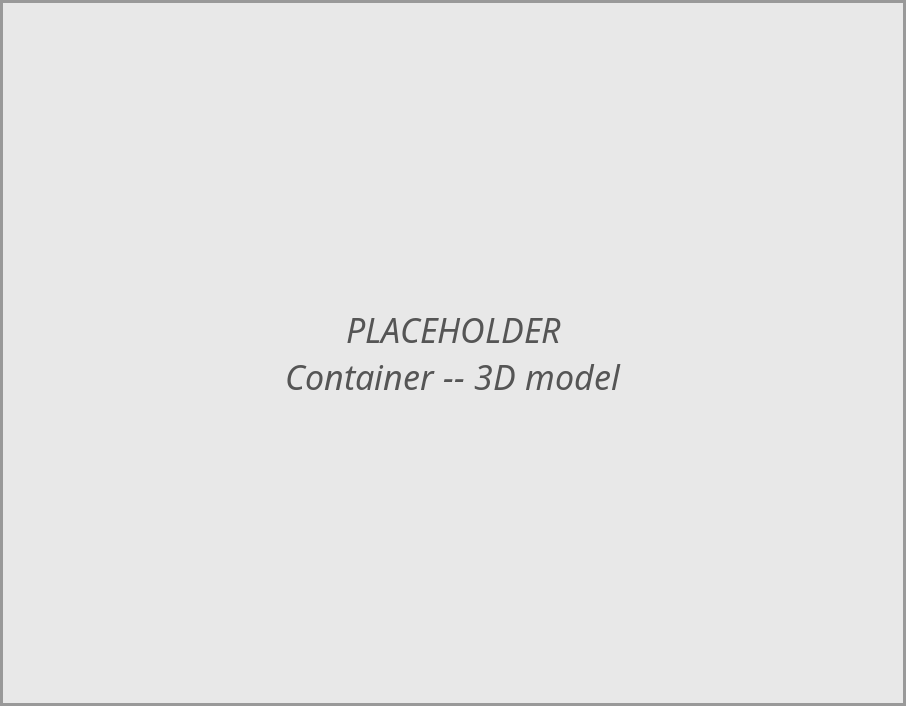
\includegraphics[height=3.5cm, keepaspectratio]{teams/science/figures/container_3d_model}
    \end{minipage}
    \hfill
    \begin{minipage}[c]{0.49\textwidth}
        \centering
        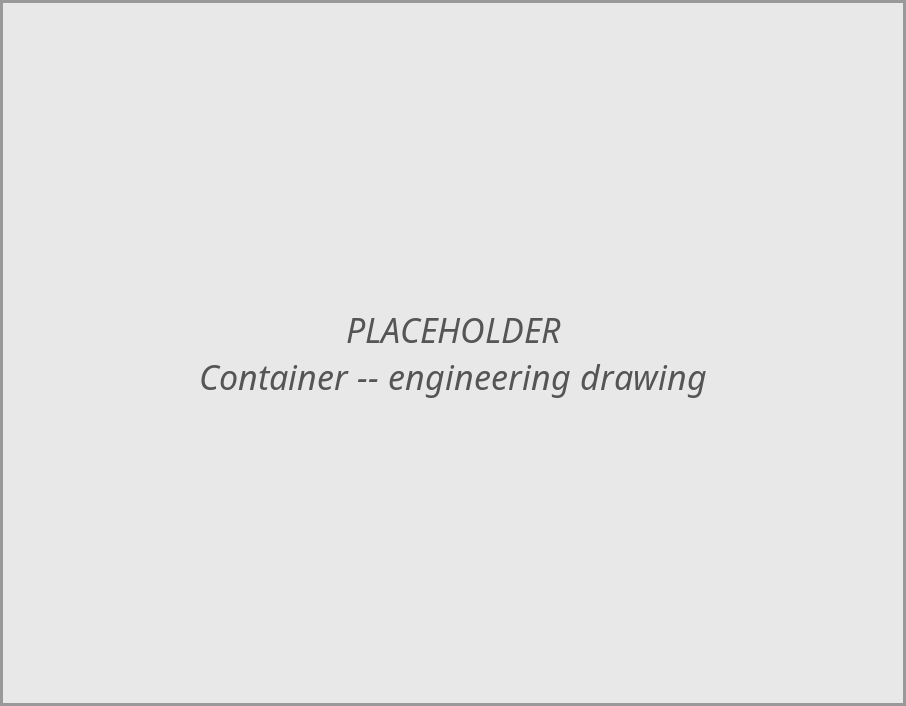
\includegraphics[height=3.5cm, keepaspectratio]{teams/science/figures/container_drawing}
    \end{minipage}

    \caption{Sample storage container: 3D model (left) and engineering drawing (right)}
    \label{fig:science_container_scheme}
\end{figure}

\begin{figure}[!htbp]
    \centering
    \setlength{\fboxsep}{0pt}

    \begin{minipage}[c]{0.49\textwidth}
        \centering
        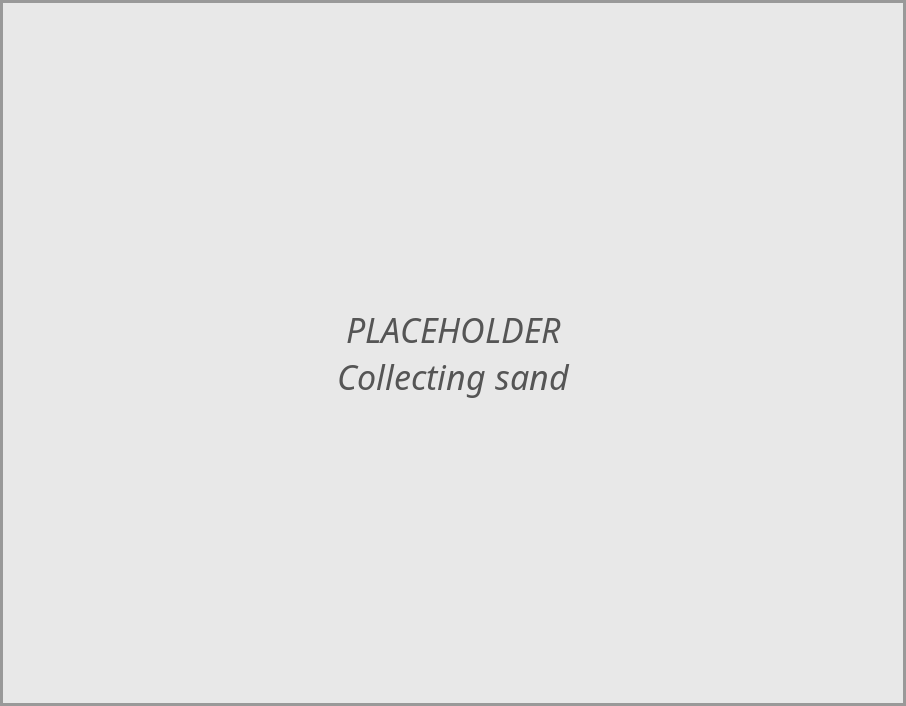
\includegraphics[height=3.5cm, keepaspectratio]{teams/science/figures/collecting_sand}
    \end{minipage}
    \hfill
    \begin{minipage}[c]{0.49\textwidth}
        \centering
        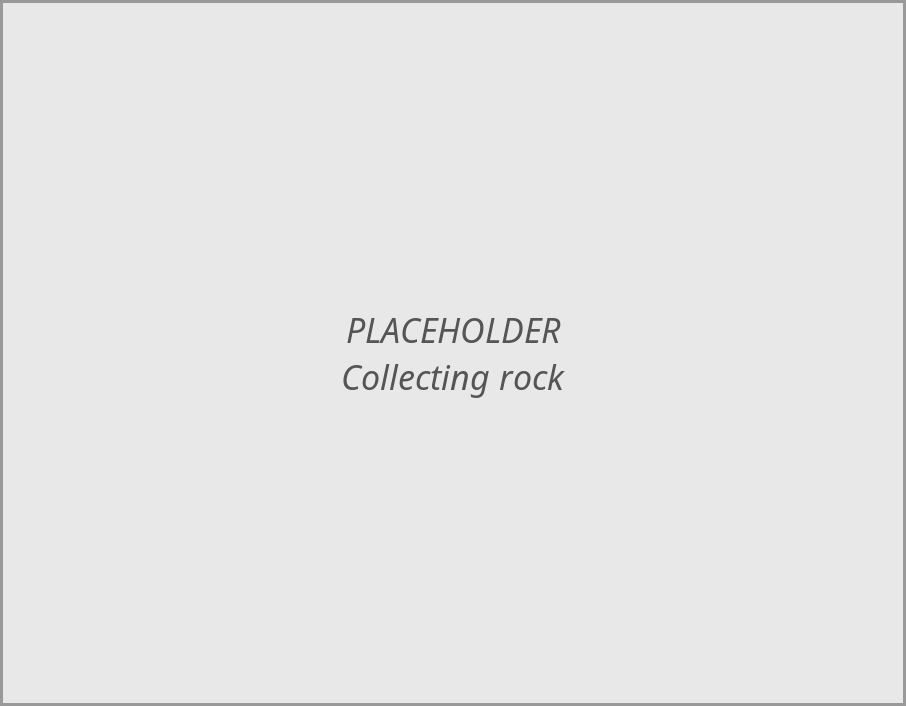
\includegraphics[height=3.5cm, keepaspectratio]{teams/science/figures/collecting_rock}
    \end{minipage}

    \caption{Science container in use: collecting regolith (left) and a rock specimen (right)}
    \label{fig:science_container_action}
\end{figure}
